%%=============================================================================
%% Methodologie
%%=============================================================================

\chapter{\IfLanguageName{dutch}{Methodologie}{Methodology}}%
\label{ch:methodologie}

%% TODO: Hoe ben je te werk gegaan? Verdeel je onderzoek in grote fasen, en
%% licht in elke fase toe welke stappen je gevolgd hebt. Verantwoord waarom je
%% op deze manier te werk gegaan bent. Je moet kunnen aantonen dat je de best
%% mogelijke manier toegepast hebt om een antwoord te vinden op de
%% onderzoeksvraag.

\section{Analyse}
De bestaande AI-tools (tijdens de periode van de literatuurstudie) worden aandachtig doorlopen en direct op de proef gesteld door (stukken van) een webshop van de co-promotor zijn lijst na te maken als template. Deze templates moeten zo dicht mogelijk aanleunen bij het gewenste resultaat (de oorspronkelijke webshop). Vervolgens bekijken we of de AI-tools in staat zijn om data te voorzien op deze templates.

\subsection{Lijst van AI-tools}
Volgende AI-tools worden gebruikt voor het overnemen van lay-out en data:
\begin{itemize}
    \item ChatGPT (op moment van schrijven zeer onstabiel)
    \item CopyAI (op moment van schrijven weinig werkende opties)
    \item 10Web (exporteren helaas niet mogelijk)
    \item Bing AI (toegang gekregen op 17/03)
    \item AgentGPT (op moment van schrijven zeer onstabiel)
\end{itemize} 

\subsection{Criteria}
De AI-tools kunnen met elkaar vergeleken worden op basis van heel wat meetbare aspecten. Aangezien de AI-evolutie deze constant beïnvloedt is het aan de co-promotor zelf om hierin een besluit te trekken. Een aantal van deze aspecten zijn:
\begin{itemize}
    \item de prijs
    \begin{itemize}
        \item gratis
        \item betalend met een eenmalige kost
        \item betalend met abonnement (in verschillende types)
    \end{itemize} 
    \item de uitvoeringssnelheid
    \begin{itemize}
        \item traag
        \item normaal
        \item snel
        \item snel (tegen betaling)
    \end{itemize} 
    \item de export limieten
    \begin{itemize}
        \item exporteerbaar
        \item enkel gebruik binnen AI-tool
    \end{itemize}
    \item integratie met een CMS
    \begin{itemize}
        \item niet mogelijk
        \item mogelijk voor WordPress
        \item mogelijk maar niet voor WordPress
    \end{itemize}
    \item automatisch opvullen van data
    \begin{itemize}
        \item mogelijk
        \item niet mogelijk
    \end{itemize}
    \item ...    
\end{itemize} 

\subsection{De webshops van de co-promotor}
De co-promotor heeft volgende lijst van webshops meegegeven:
\begin{itemize}
    \item Coureur Local
    \item A bloc
    \item Angar
    \item Mr. Teddybeer
    \item Wittevrongel
    \item Petites Jubelles
    \item Kwiek en kwispel
    \item My shirt matters
    \item Motorcycle cushions
\end{itemize} 

\subsection{Scenario's}
De mogelijke scenario's die kunnen optreden bij het overnemen van een webshop zijn als volgt:
\begin{itemize}
    \item Geen WordPress
    \begin{itemize}
        \item toegang tot MySQL databank
        \item geen toegang tot MySQL databank
        \item geen MySQL databank
        \begin{itemize}
           \item overzetten naar MySQL
           \item niet kunnen overzetten
       \end{itemize} 
    \end{itemize}
    \item Wel WordPress 
    \begin{itemize}
        \item toegang tot de site
        \begin{itemize}
            \item toegang tot de databank
            \begin{itemize}
                \item met WooCommerce export
                \item zonder WooCommerce export
            \end{itemize} 
            \item geen toegang tot de databank
            \begin{itemize}
                \item met WooCommerce plugin actief
                \item zonder WooCommerce plugin actief
            \end{itemize} 
        \end{itemize} 
        \item geen toegang tot de site
        \begin{itemize}
            \item met WooCommerce plugin actief
            \item zonder WooCommerce plugin actief
        \end{itemize} 
    \end{itemize} 
\end{itemize} 

\section{Installatie van WordPress}
Het installeren van een WordPress instantie verloopt in een aantal stappen die geautomatiseerd kunnen worden. In volgende hoofdstukken worden deze besproken voor de webshop Coureur Local. Aangezien de co-promotor met Windows werkt zullen alle scripts en terminal commands geschreven zijn in Powershell.

\subsection{Folderstructuur}
In een WordPress installatie zijn verschillende folders aanwezig die elk hun eigen functionaliteit hebben. De belangrijkste hiervan zijn:
\begin{itemize}
    \item wp-admin - hierin komt alle code te staan die specifiek voor de administrator is zoals het dashboard
    \item wp-content - deze map één van de belangrijkste en zal hieronder verder besproken worden
    \item wp-includes - hierzin zitten de basis functionaliteiten om de CMS te doen werken
\end{itemize} 

\subsection{De wp-content}
Bij het opstellen van een nieuwe webshop zal deze folder de meeste aanpassen krijgen. De belangrijkste subfolders hier zijn:
\begin{itemize}
    \item plugins - elke plugin wordt in deze folder geïnstalleerd
    \item themes - hierin komen de standaard WordPress-themes alsook de eigen custom themes terecht
    \item uploads - hierzin zitten alle mediabestanden zoals afbeeldingen en video's die worden geüpload 
\end{itemize} 

\subsection{Databank en sitegegevens}
Command-line tools of scripts kunnen de downloadlink van WordPress ophalen, het zipbestand downloaden en automatisch uitpakken naar de juiste locatie. WordPress werkt op een MySQL-databank, de aanmaak hiervan kan ook worden geautomatiseerd met behulp van scripts. Tenslotte kunnen een aantal webshop-gegevens reeds voorzien worden zoals de website titel, beschrijving, tijdzone en taal. Een standaard gebruiker instellen kan via deze weg ook. Merk op dat er nog meer instellingen kunnen aangevuld worden zoals de adminEmail, permalinkStructure, uploadsPath, defaultCategory enzovoort.

\subsection{Custom theme}
WordPress werkt met thema's om de lay-out en design van een website te bewaren. Standaard installeert en activeert WordPRess een thema van hen. Een custom theme is een thema dat je volledig zelf in beheer hebt. Dit geeft het voordeel van een volledig uniek design te implementeren, maar vergt bijgevolg wel meer kennis. Er zijn verschillende opties voor de co-promotor:
\begin{itemize}
    \item WordPress thema - blijf met het standaard thema werken
    \item eigen custom theme - maak zelf een custom theme (per project) aan
    \item download een custom theme - haal een (betalende) custom theme van het internet af en bewerk die
\end{itemize}
Voor veiligheidsredenen is het aangeraden om altijd een standaard WordPress thema gedownload te hebben. Mocht er een fout optreden met een custom theme dan kan WordPress daarop terugvallen. Het zal mogelijks voor een andere lay-out zorgen, maar de website zal geen foutmelding geven of zelfs niet beschikbaar zijn. 

\subsection{WP-CLI}
Om de veiligheid en toekomstige compatibiliteit van het script te verbeteren kan men best werken met de WP-CLI (WordPress Command Line Interface) tool. Het is veiliger omdat het gebruik maakt van de ingebouwde WordPress-beveiliging om ervoor te zorgen dat de ingevoerde gegevens worden gevalideerd. Dit helpt potentiële beveiligingsproblemen zoals SQL-injecties te voorkomen. Doordat het gebruik maakt van de officiële WordPress-cli-functionaliteit is het minder waarschijnlijk dat het wordt beïnvloed door toekomstige updates of wijzigingen in de WordPress-codebase, en het langer zal blijven werken met toekomstige versies van WordPress.
\\\\
De WP-CLI maakt gebruik van wp option update commando's. Om wp option update te gebruiken in een script, moet je eerst zorgen dat WP-CLI is geïnstalleerd op je systeem en dat het beschikbaar is in het pad (PATH).
\\\\
Hiervoor is PHP 5.4.0 of hoger nodig. De versie kan je controleren in de terminal met volgend commando:
\begin{minted}{bash}
php --version
\end{minted}
Indien je geen antwoord krijgt dan moet je PHP nog installeren. Vervolgens moet je \href{https://wp-cli.org/#installing}{WP-CLI} downloaden en installeren.. Tenslotte moet je het pad van wp-cli nog toevoegen aan de omgevingsvariable PATH op jouw systeem. Je kan controleren of alles goed werkt door info op te halen via het commando:
\begin{minted}{bash}
wp --info
\end{minted}

\subsection{Voorbeeldscript configuratiebestand}
Wachtwoorden en andere gevoelige gegevens worden best veilig opgeslagen in een aparte configuratiebestand en worden best niet zomaar weergegeven in een script. Het grote voordeel aan deze werkwijze is dat alle noodzakelijke gegevens voor de installatie op één centrale plaats komen te staan. Op de \href{https://wordpress.org/documentation/article/settings-general-screen/}{WordPress website} kunnen alle mogelijke settings om aan te passen worden teruggevonden. Een voorbeeld van zo een configuratiebestand in PowerShell:
\begin{minted}{bash}
#!/bin/bash
# Configuratiebestand voor WordPress-installatie

# Database-instellingen
dbHost="localhost"
dbPort="3306"
dbUser="db_username"
dbPassword="db_password"
dbName="db_name"

# Site-instellingen
siteTitle="Coureur Local"
siteDescription="Koop bij ons jouw nieuwe fiets."
siteTimezone="Europe/Amsterdam"
siteLanguage="nl_NL"
siteUrl="https://coureurlocal.be"

# Standaard gebruiker instellen
defaultUsername="Admin"
defaultPassword="admin_wachtwoord"

# WordPress-map pad
wordpressPath="$HOME/Desktop/webshops/coureur_local/"

# Thema instellingen
author="Team Made"
themesPath="$HOME/Desktop/webshops/coureur_local/wp-content/themes"
themeName="Thema Coureur Local"
themeDescription="Thema speciaal voor Coureur Local gemaakt."

# Exporteer variabelen voor gebruik in andere scripts
export dbHost
export dbPort
export dbUser
export dbPassword
export dbName
export siteTitle
export siteDescription
export siteTimezone
export siteLanguage
export siteUrl
export defaultUsername
export defaultPassword
export wordpressPath
export author
export themesPath
export themeName
export themeDescription
\end{minted}


\subsection{Voorbeeldscript algemene opzet}
Een voorbeeld van een script in PowerShell voor WordPress automatisch te installeren, de databasegegevens in te vullen en een standaard gebruikersaccount aan te maken:
\begin{minted}{powershell}
# Laden van configuratiebestand
$config = Get-Content -Path "config.ps1" | ConvertFrom-StringData

# Downloaden en uitpakken van WordPress
Invoke-WebRequest -Uri "https://wordpress.org/latest.tar.gz" -OutFile "latest.tar.gz"
Expand-Archive -Path "latest.tar.gz" -DestinationPath $config.wordpressPath

# Kopiëren van WordPress-bestanden naar de gewenste locatie
Copy-Item -Path "wordpress\*" -Destination $config.wordpressPath -Recurse

# Configuratiebestand aanmaken
Copy-Item -Path "$($config.wordpressPath)\wp-config-sample.php" -Destination "$($config.wordpressPath)\wp-config.php"

# Invullen van databasegegevens in het configuratiebestand
(Get-Content -Path "$($config.wordpressPath)\wp-config.php") |
ForEach-Object {
    $_ -replace "'DB_HOST', 'localhost'", "'DB_HOST', '$($config.dbHost)'" `
    -replace "'DB_PORT', '3306'", "'DB_PORT', '$($config.dbPort)'" `
    -replace "'DB_USER', 'db_username'", "'DB_USER', '$($config.dbUser)'" `
    -replace "'DB_PASSWORD', 'db_password'", "'DB_PASSWORD', '$($config.dbPassword)'" `
    -replace "'DB_NAME', 'db_name'", "'DB_NAME', '$($config.dbName)'" `
} | Set-Content -Path "$($config.wordpressPath)\wp-config.php"

# Aanpassen van bestandseigenaar en -groep (optioneel)
if ($config.chownEnabled) {
    $acl = Get-Acl $config.wordpressPath
    $acl.SetOwner([System.Security.Principal.NTAccount]("IIS APPPOOL\$($config.appPoolUser)"))
    Set-Acl -Path $config.wordpressPath -AclObject $acl
}

# Bijwerken van WordPress-site instellingen
Set-ItemProperty -Path "$($config.wordpressPath)\wp-config.php" -Name "siteurl" -Value $config.siteUrl
Set-ItemProperty -Path "$($config.wordpressPath)\wp-config.php" -Name "blogname" -Value $config.siteTitle
Set-ItemProperty -Path "$($config.wordpressPath)\wp-config.php" -Name "blogdescription" -Value $config.siteDescription
Set-ItemProperty -Path "$($config.wordpressPath)\wp-config.php" -Name "timezone_string" -Value $config.siteTimezone
Set-ItemProperty -Path "$($config.wordpressPath)\wp-config.php" -Name "WPLANG" -Value $config.siteLanguage

# Verwijderen van WordPress-archief
Remove-Item "latest.tar.gz"

Write-Host "WordPress is geïnstalleerd, databasegegevens zijn automatisch ingevuld en een standaard gebruikersaccount is aangemaakt."
\end{minted}
\subsection{Voorbeeldscript custom theme}
Indien er gekozen wordt om een volledig nieuw custom theme aan te maken en te activeren, kan dit ook met behulp van scripting.
Een voorbeeld van een PowerShell script voor het aanmaken en activeren van een custom theme dat opnieuw gebruik maakt van een configuratiebestand:
\begin{minted}{bash}
# Import the configuration file
$configFilePath = "C:\path\to\config.ps1"  # Path to the configuration file
$config = Get-Content -Path $configFilePath -Raw | Invoke-Expression

# Retrieve the values from the configuration
$wordpressPath = $config.wordpressPath
$author = $config.author
$themesPath = $config.themesPath
$themeName = $config.themeName
$themeDescription = $config.themeDescription

# Create the custom theme folder
$themeFolderPath = Join-Path -Path $themesPath -ChildPath $themeName
New-Item -Path $themeFolderPath -ItemType Directory -Force

# Add a sample image to the theme folder
$sampleImage = "C:\path\to\sample-image.jpg" 
$destinationImagePath = Join-Path -Path $themeFolderPath -ChildPath "sample-image.jpg"
Copy-Item -Path $sampleImage -Destination $destinationImagePath -Force

# Create the necessary theme files
$styleFilePath = Join-Path -Path $themeFolderPath -ChildPath "style.css"
$indexFilePath = Join-Path -Path $themeFolderPath -ChildPath "index.php"

# Generate the content for the style.css file
$styleContent = @"
/*
Theme Name: $themeName
Description: $themeDescription
Version: 1.0
Author: $author
*/

/* Additional CSS styles go here */
"@
$styleContent | Set-Content -Path $styleFilePath

# Generate the content for the index.php file
$indexContent = @"
<?php
// Silence is golden.
"@
$indexContent | Set-Content -Path $indexFilePath

# Activate the custom theme
$command = "& `"$wordpressPath\wp-cli.phar`" --path=`"$wordpressPath`" theme activate $themeName"
Invoke-Expression $command

# Output success message
Write-Host "Custom theme '$themeName' is geïnstalleerd en geactiveerd"
\end{minted}
Via deze weg kan heel eenvoudig per klant een custom theme worden aangemaakt door enkel het configuratiebestand manueel in te vullen, en een afbeelding te voorzien.

\subsection{Voorbeeldscript plugins}
Eens een WordPress installatie volledig opgezet is dan kan een admin zich inloggen en visueel plugins beheren. Het is echter ook mogelijk om via scripting een plugin te downloaden en vervolgens te installeren in de WordPress-installatie. Deze nieuwe plugin komt dan ook terecht in de directory /wp-content/plugins. Ook dit bespaart manueel werk als op voorhand reeds geweten is welke plugin(s) zullen worden gebruikt.
\\\\
Belangrijk om in het achterhoofd te houden is dat plugins geschreven zijn door mensen die (meestal) niet per se van WordPress zelf zijn. Hou er rekening mee dat plugins beveiligingsrisico's met zich meenemen en mogelijks uw webshop kwetsbaar kunnen maken zoals Advanced Custom Fields (Pro) die in oudere versies XSS-aanvallen toelaat \autocite{Leemputten2023}. Het is aan de programmeur om te bepalen welke versie je neemt van de plugin, en of je de plugins automatisch laat updaten door WordPress of niet. Een mogelijke reden om niet automatisch te willen updaten kan het breken van compatibiliteit met andere plugins of andere WordPress functionaliteiten zijn.
\\\\
Een voorbeeld van een PowerShell script voor het downloaden en installeren van de WooCommerce plugin:
\begin{minted}{bash}
# Import the configuration file
$configFilePath = "C:\path\to\config.ps1"
$config = Get-Content -Path $configFilePath -Raw | Invoke-Expression

# Retrieve the value of the wordpressPath variable from the configuration
$wordpressPath = $config.wordpressPath

$pluginsPath = Join-Path -Path $wordpressPath -ChildPath "wp-content\plugins"  

# WooCommerce plugin download URL
$woocommerceUrl = "https://downloads.wordpress.org/plugin/woocommerce.latest-stable.zip" 

# WooCommerce plugin name and file name
$woocommerceName = "woocommerce"  # Name of the WooCommerce plugin
$woocommerceFileName = "$woocommerceName.zip"  # Name of the downloaded ZIP file

# Download WooCommerce plugin
$woocommerceFilePath = Join-Path -Path $PSScriptRoot -ChildPath $woocommerceFileName
Invoke-WebRequest -Uri $woocommerceUrl -OutFile $woocommerceFilePath

# Extract WooCommerce plugin
Expand-Archive -Path $woocommerceFilePath -DestinationPath $pluginsPath -Force

# WordPress Plugin API activation
$apiPath = Join-Path -Path $wordpressPath -ChildPath "wp-load.php"
Import-Module $apiPath

# Activate WooCommerce plugin using Plugin API
$pluginPath = Join-Path -Path $pluginsPath -ChildPath $woocommerceName 
activate_plugin($pluginPath)

# Output success message
Write-Host "WooCommerce plugin is gedownload, geïnstalleerd en geactiveerd."
\end{minted}
Indien gewenst is het mogelijk om de automatische updates van WordPress direct aan te zetten door het script uit te breiden met:
\begin{minted}{bash}
$command = "& `"$wordpressPath\wp-cli.phar`" --path=`"$wordpressPath`" eval 'add_filter( ""auto_update_plugin"", ""__return_true"" );'"
Invoke-Expression $command
\end{minted}
Ook voor dit script halen we de configuratiebestand op voor het pad naar de WordPress installatie te achterhalen. Natuurlijk kan ook gekozen worden om het plugin pad hierin te steken. Plugins kunnen ook een activeerscript hebben, maar de paden hiervan kunnen variëren van plugin tot plugin. Dit probleem los je op door met de WordPress Plugin API te werken. Merk op dat het commando 'Active-Plugin' de WordPress Plugin API nodig heeft, die in de wp-load.php zit. Afhankelijk van de co-promotor zijn voorkeuren kan hij ervoor kiezen om:
\begin{itemize}
    \item per plugin een script te schrijven, en die één voor één te laten uitvoeren
    \item een combinatie van (veelgebruikte) plugins in één script te steken, om per project eenmalig uit te voeren
    \item alle scripts tot één script te combineren
    \item ...
\end{itemize} 
De auteur raadt aan om te wachten met het installeren van plugins in verband met beveiliging totdat de webshop live staat. Dit omdat deze plugins (bv. Wordfence) een firewall installeren, die bij het deployen van een webshop dubbel werk kunnen geven.
\section{Styling van lay-out}
Indien er voor een custom theme wordt gekozen en de styling volledig vanaf nul moet worden overgenomen, zijn er op moment van schrijven weinig AI-tools om daarbij te helpen. Het grote probleem is dat afbeelding-herkenningen nog niet aanwezig zijn in de publiek toegankelijk AI-tools. Deze zouden echter de beste oplossing zijn voor dit probleem. Naar toekomstig gebruik toe kan een gebruiker op basis van een screenshot vragen om het in code om te zetten. Op moment van schrijven moet de gebruiker zelf zeer duidelijk specifiëren wat hij wilt, wat zeer omslachtig is. Daarom is het sterk aangeraden om voor deze stap nog met een front-end developer te werken.

\section{Overname van data}
Voor het ophalen van goederen en/of diensten hun data zijn er verschillende opties aanwezig. Voor de auteur was het op moment van schrijven niet mogelijk om op de beta versie alle functionaliteiten van AgentGPT te testen, maar webscraping bleek wel (in beperkte mate) goed te werken. Indien dit in de toekomst blijft werken (of zal verbeteren) is dit een zeer gebruiksvriendelijke werkwijze om zonder extra tools data van een webpagina op te halen. Merk op dat AgentGPT gebruik maakt van een Python bibliotheek \href{https://www.crummy.com/software/BeautifulSoup/bs4/doc/}{Beautiful Soup} om data op te halen van een webpagina (zie figuur 3.1). 
\begin{figure}
    \caption{'AgentGPT gebruikt BeautifulSoup voor het ophalen van data op een webpagina'}
    \begin{center}
        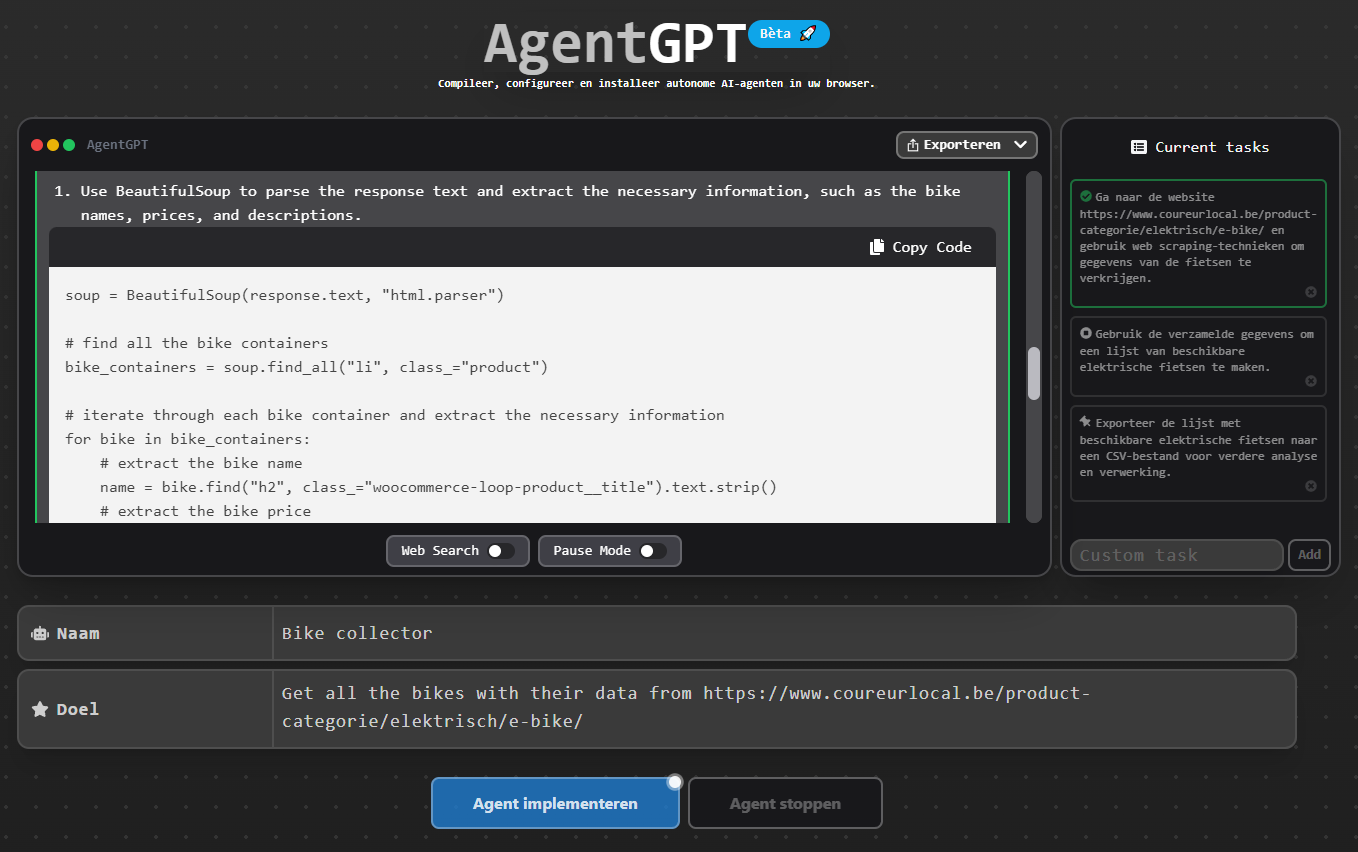
\includegraphics[width=\textwidth, height=\textheight, keepaspectratio]{agentgpt_uses_beautifulSoup}
    \end{center}
\end{figure} 
\\\\
ChatGPT kan op moment van schrijven al bestaande data omzetten naar nieuwe type data. Hiermee kan je een .csv-file aanmaken met de verkregen data, mocht die nog niet in een .csv-file zitten, om vervolgens te \href{https://woocommerce.com/document/importing-woocommerce-sample-data/}{importeren met in de WooCommerce plugin}.